\chapter{Design and Architecture}
\label{chap:design-and-architecture}


\section{Using FUSE in C++}\label{sec:fuse-in-cpp}

Properly incorporating FUSE in C++ presents many design challenges, primarily due to its interface design, which necessitates the use of a static wrapper for operations.
The problem arises from FUSE expecting a C struct with pointers to functions, which poses a problem for non-static C++ methods.
To solve this issue, two solutions can be considered: either writing C++ code without utilizing objects, rendering the use of C++ instead of C rather pointless, or implementing a singleton wrapper with only static methods.

As is evident, the latter solution was chosen.
Fortunately, there was no need to start from scratch, as existing repositories already provide a solution to this problem.
However, none of them were complete and up-to-date, and I still had to write some portion of the code myself.

The foundation for this project was built upon the fusexx~\cite{fusexx} repository, which was found most suitable for the needs of this thesis.
But as I said, significant changes were made to the existing code, as it was not written in a modern C++ style and did not adhere to the project's design goals.
The first step was therefore to refactor the code to use modern C++ features and resolve numerous clang-tidy warnings.
Moreover, the repository was not updated for several years, and it was necessary to change some of the code's version-specific parts.
And as a final touch, some methods were completely rewritten to improve readability or efficiency.

Needless to say, there was also a third, rather ``hacky'' solution, more like a sub-solution of the second one, which involved beside other implementation details using a data field in the FUSE context to store a pointer to the C++ object.
Something similar is done in the fusepp~\cite{fusepp} repository.
But this approach did not seem to be the most elegant solution, and it was decided to use the singleton wrapper instead.
Furthermore, the fusepp repository was not updated for even longer and would be harder to be used as a base for the project.


\section{Architecture}\label{sec:architecture}

Once the foundation was laid; the next step was to design a core VFS\@.
It is important to note that this implementation was not the primary focus of this thesis as it was rather focused on providing modularity and extensibility.
The result of this is that the entire core VFS is built on top of already present filesystem in the operating system.
It is based on simply using a backing directory to store all the files and directories.
However, such implementation details can be easily replaced, allowing for future improvements.

Still, there were some design decisions to be made regarding the object-oriented design of the VFS\@.
And multiple approaches were contemplated: mainly one involving a single VFS class and another comprising separate File, Directory, and VFS classes.
Although the latter approach adheres more closely to object-oriented principles, I have decided to go with the former, as it is better suited for use with FUSE\@.
The reason for that is I would still need to somehow bound all those classes into one, meaning at least the wrapper would have to be more complicated.
Another concern regarding the second approach is that it would be harder to make the VFS extensible, but more on that in the following sections.

\subsection{Modularity}\label{subsec:modularity}

The VFS is designed to be modular, allowing for the addition of new features without the need to modify the core implementation.
To achieve this, the decorator pattern was selected as the primary design pattern for this project.

The decorator pattern is a structural design pattern that involves a set of decorator classes used to wrap concrete components.
Decorator classes mirror the types of the components they decorate, sharing the same interface but adding or overriding behavior.

The benefit of this pattern is that it allows for the dynamic addition of new features to an object without modifying its implementation.
Also, it is possible to combine multiple decorators to add multiple features to the same object at the same time.
These properties make the decorator pattern a perfect fit for this project.

The decorator pattern is thus used to implement the VFS prototypes, such as encryption and versioning.
For example, an \texttt{EncryptionVfs} class is implemented as a decorator, inherited from the \texttt{VfsDecorator} class.
The \texttt{VfsDecorator} class, in turn, inherits from the base \texttt{CustomVfs} class.
The decorator class wraps an instance of the base VFS class, allowing it to perform additional encryption-related tasks when reading or writing files.

Following code snippet showcase the standard implementation of decorator pattern:

\begin{lstlisting}[language=c++, caption={Decorator pattern implementation},basicstyle=\ttfamily\small]
class CustomVfs { /.../ };

class VfsDecorator : public CustomVfs {
public:
explicit VfsDecorator(CustomVfs& wrapped_vfs);

protected:
CustomVfs& wrapped_vfs_;
};

class EncryptionVfs : public VfsDecorator {
public:
explicit EncryptionVfs(CustomVfs& wrapped_vfs);

int read(/.../) override;
int write(/.../) override;
};
\end{lstlisting}

It's important to note that I currently do use both inheritance and composition in the decorator pattern.
The reason behind that is that it allows me to spare some boilerplate code and make the code more readable as I use the CustomVfs more like a value type (if there was such thing in C++), meaning its behaviour is defined not by its reference but the values inside it.
This allows me to simply copy construct the parent \texttt{CustomVfs} object with passed decorator.

The use of this pattern is then demonstrated in the following code snippet, which shows how the VFS is initialized and used in the \texttt{main} function:

\begin{lstlisting}[language=c++, caption={VFS initialization and usage},basicstyle=\ttfamily\small]
int main(int argc, char* argv[]) {
    CustomVfs custom_vfs();
    VersioningVfs versioned_vfs(custom_vfs);
    EncryptionVfs enc_vers_vfs(versioned_vfs);

    enc_vers_vfs.main(argc, argv);
    return 0;
}
\end{lstlisting}

Anyone can easily add new features to the VFS by implementing a new decorator class and wrapping it around the base VFS\@.

\subsection{Modularity caveats}\label{subsec:modularity-cavs}

Unfortunate thing about this modularity design is complications with accessing the files other ways than using the parent decorator.
To demonstrate my point, I will explain the complication with combing versioning and encryption.
With that, you have to consider what do you want to perform first.
In case of first versioning and then encryption, you have to encrypt all the concerned files.
In case of first encrypting and then versioning, you lose the ability to version the diff-based way.

This order decision has to be done by the person creating the result vfs, but it is my responsibility to provide sufficient tools.
For the described example, it means simply that each decorator has to be able to ask its parent for all concerned files.

\subsection{Access to VFS features}\label{subsec:access-to-vfs-features}

Another crucial aspects of the architecture is determining the method by which users can access the added VFS features.
In this implementation, hooks have been designed to integrate seamlessly with standard filesystem operations.
What I mean by a hook is a file with a specific name that triggers a specific action when accessed.
Additionally, a simple command-line interface (CLI) has been implemented to facilitate creating hooks for the VFS features.

The filesystem captures the mentioned operation, performs the requested action, and returns the result of the operation to the user.
This approach allows users to interact with the VFS features without deviating from standard filesystem operations.

The CLI consists of two primary components: one for encryption and another for versioning.
Users can execute commands related to these features via the CLI, making it a user-friendly and accessible interface for interacting with the VFS\@.
Commands for encryption may include encryption key management and selecting encryption algorithms, while versioning commands may involve creating new versions, listing available versions, and reverting to a previous version.

Although the current implementation utilizes a command-line interface, the hooks can potentially be integrated into a graphical user interface (GUI) in the future.
Incorporating the VFS features into a GUI would provide users with an even more intuitive and visually appealing interface for managing encryption and versioning.
However, the development of a GUI was beyond the scope of this thesis.

Benefits of this approach include the ability to easily integrate the VFS features into existing applications, such as file managers.
This is because the VFS features are accessed through standard filesystem operations, which are already supported by most applications.
Additionally, the hooks allow for the seamless integration of new features, such as encryption and versioning, without the need to modify the core VFS implementation as can be seen in the following code example:

\begin{lstlisting}[language=c++, caption={Example of hook implementation}, basicstyle=\ttfamily\small]
int Vfs::write(const std::string &ppath, char *buffer,
               size_t size, off_t offset) {
    if (is_hook(path)) {
        return handle_hook(path, buffer, size, offset);
    }

    // Do normal write operation...
}
\end{lstlisting}

Each module has then its own implementation.
It is also necessary to mention that I use one format for all hooks, which starts with a special character and then is followed by the name of the hook.
For this reason, the module needs to be able to ignore hooks that are not meant for it.

\subsection{Architectural overview}\label{subsec:overview}

I will conclude this chapter by providing an architectural overview of the VFS\@.
The architecture of our system is designed using object-oriented principles to ensure modularity, extensibility, and maintainability.
The core of the system is built around the FuseWrapper class, which provides a base implementation for interacting with the FUSE library.
By deriving from this base class, we can create custom virtual file systems with various features and functionality.

The CustomVfs class inherits from FuseWrapper and serves as a foundation for more specialized virtual file systems.
By utilizing the decorator pattern, we implement additional functionality in separate classes, such as EncryptionVfs and VersioningVfs, which both inherit from the VfsDecorator class.
This approach allows us to easily extend the system with new features while minimizing the impact on existing code.

The key components of the architecture, along with their relationships and key methods, are illustrated in Figure~\ref{fig:uml_diagram}.
The diagram shows the main classes, their inheritance relationships, and some of the methods that define their behavior.

Still, there are a lot of helper classes that are not shown in the diagram, but they are not important for the understanding of the architecture.
These classes would typically include logging, handling paths or custom tool for prefixing file names with custom metadata.

\begin{figure}[ht]
    \centering
    \scalebox{1}{
        
\begin{tikzpicture}
    \umlclass[x=0, y=0]{FuseWrapper}{
        + static struct fuse\_operations ops
    }{
        + main(\ldots) \{\ fuse\_main(\ldots, \&ops, this);\ \} \\
        \\
        + virtual write(\ldots) \\
        + virtual read(\ldots) \\
        + virtual open(\ldots) \\
        + \ldots
    }

    \umlclass[x=0, y=-5.2]{CustomVfs}{
        -- std::string mountpoint \\
        -- std::string backing\_dir
    }{
        + write(\ldots) \\
        + read(\ldots) \\
        + open(\ldots) \\
        + main(\ldots) \\
        + \ldots
    }

    \umlclass[x=0, y=-9]{VfsDecorator}{
        -- CustomVfs\& wrapped\_vfs
    }

    \umlclass[x=-2, y=-11.7]{EncryptionVfs}{
    }{
        + write(\ldots) \\
        + read(\ldots) \\
        \# encrypt(\ldots) \\
        \# decrypt(\ldots) \\
        \ldots
    }

    \umlclass[x=2, y=-11.7]{VersioningVfs}{
    }{
        + write(\ldots) \\
        + read(\ldots) \\
        \# revert(\ldots) \\
        \ldots
    }

    \umlinherit{CustomVfs}{FuseWrapper}
    \umlinherit{VfsDecorator}{CustomVfs}
    \umlinherit{EncryptionVfs}{VfsDecorator}
    \umlinherit{VersioningVfs}{VfsDecorator}
\end{tikzpicture}
    }
    \vspace{15pt}
    \caption{UML diagram of the system architecture.}
    \label{fig:uml_diagram}
\end{figure}